%tudo o que está a seguir a esta percentagem nao é comentado, assim se faz comentarios no "código" em latex

\documentclass[a4paper,11pt]{report}%deve ser sempre a primeira linha de codigo num documento em latex,define-se o tipo de documento "article"(1), tamanho de folha "a4paper" e o tamanho de letra "9pt". Estes parametros são necessários para uma correta modelação e impressão do documento em questão
% (1)
% {article} - artigos, pequenos relatorios,documentação de programas, convites
% {report} - relatorios mais complexos, contendo varios capitulos, pequenos livros, testes de doutoramento
% {book} - o nome diz tudo
% {slides} - o nome diz tudo

\usepackage[portuguese]{babel} %para traduzir todo o conteudo da estrutura documental para portugues

\usepackage[utf8]{inputenc}%para abilitar acentuação e uso de carateres especiais
% \usepackage[latin1]{inputenc}%alternativa para abilitar acentuação e uso de carateres especiais

\usepackage{verbatim} %Para criar comentários de múltiplas linhas (alternativa ao % que só funciona para uma linha), primeiros devemos incluir o pacote chamado verbatim, normalmente usado para incluir códigos fonte no seu documento.

\usepackage{fancyhdr} %para poder usar o fancy, isto é, criar caso necessário o meu proprio cabeçalho

\usepackage{indentfirst} %caso o objectivo é indentar a primeira linha do parágrafo, isto é, usar o,\indent
%todo o que está para traz, diz respeito apenas a configurações e bibliotecas necessárias para aplicar formatações ao ficheiro a ser criado


\usepackage{listings} %este pacote é usado para poder interpretar os exertos de código como se estivessem a ser apresentados no IDE
\lstdefinestyle{customc}{%tudo o que se encontra dentro destas chavetas é para definir as cores a atribuir a cada detalhe dos extratos de codigo colocados na documentação
  belowcaptionskip=1\baselineskip,
  breaklines=true,
  frame=L,
  xleftmargin=\parindent,
  language=C,
  showstringspaces=false,
  basicstyle=\footnotesize\ttfamily,
  keywordstyle=\bfseries\color{green!40!black},
  commentstyle=\itshape\color{purple!40!black},
  identifierstyle=\color{blue},
  stringstyle=\color{orange},
}

%na linha abaixo encontra-se o parametro que deve ser colocado antes dos extratos de codigo a aplicar as definições acima atribuidas
%
%\lstset{escapechar=@,style=customc}
%
\usepackage{graphicx}% usado para podermos incorporar na documentação imagens
\begin{comment}
COM O AUXILIO DO VERBATIM COMENTO ALGUMAS EXPLICAÇÕES DE COMO USAR NESTE CASO O fancy SEM QUE ESTA EXPLICAÇÃO APAREÇA NO DOCUMENTO LATEX, PDF.

as modificações de cabeçalho a baixo deviam de funcionar o que nao se confirma, daí o fancy apenas criar um rodape padrao do mesmo
\fancypagestyle{nomeQualquer}
	{
	\fancyhead{Modelo de Latex} % a mesma coisa que o \chead 
	\fancyfoot{Rodapé Universal} % a mesma coisas que o \cfoot
	\lhead{O que quero no cabeçalho parte esquerda}
	\chead{O que quero no cabeçalho parte central}
	\rhead{O que quero no cabeçalho parte direita}
	\lfoot{O que quero no rodapé parte esquerda}
	\cfoot{O que quero no rodapé parte central}
	\rfoot{O que quero no rodapé parte direita
	}

Para iniciar uma nova linha sem iniciar um novo paragrafo usasse: \\*
Para mudar de linha a meio de uma frase, usar \newline.

Para usar aspas no latex recorre-se a duas plicas no inicio e no fim da palavra 

Quando queremos criar secções mas que estas nao apareçam no indice, basta que ao escrever \section*{blablabla} coloque um * antes do nome da secção.

\indent Assim se dá corretamente um TAB!

Quando estamos a escrever uma frase e esta sai para fora dos limites da folha, podemos fazer uma simples quebra de linha com auxilio do pipe inclinado \

\paragraph{\ } <---Assim se muda de linha devidamente (tem que ter um espaço depois da barra)

\paragraph {\ \ } <--Assim se dá espaçamento de duas linhas (tem que ter um espaço depois da barra)
Atenção que ao usar o paragraph ele muda de linha (+ espaçada) e dá-lhe um TAB na 1º linha da frase a escrever.

Por vezes é necessário fechar o pdf criado pelo latex e recompilar o documento para que o indice do mesmo seja reformulado.
\end{comment}
%++++++++++++++++++++++++++++++++++++++++++++++++++++++++++++++++++++++++++++++++++++++++++++++++++++++++++++++++++++++++++++++++++++++++++++++++++++++++++++++++
\pagestyle{fancy} %para colocar rodapé nas folhas com formatos diferentes consoante o formato escolhido, neste caso o formato escolhido é "fancy". Mas existem 3 tipos de rodapés:
% "plain" que apenas imprime o numero de pagina no fundo da mesma, 
% "headings" que imprime o nome do capitulo atual e o numero de pagina no cabeçalho de cada pagina enquanto o rodapé mantem-se vazio 
% "empty" que coloca cabeçalho e rodapé vazios.
% caso queiramos criar o nosso proprio cabeçalho e rodape usamos o "fancy"


\fancyhead{Modelo de Latex} % a mesma coisa que o \chead 
\fancyfoot{Rodapé Universal} % a mesma coisas que o \cfoot
\lhead{Nº de pagina: \thepage}
\rfoot{rodape direito}
\rhead{\today} %se quiser inserir uma data expecifica, esta deve ser literalmente escrita entre as chavetas
\lfoot{rodapé parte esquerda}
\rfoot{\rightmark}%coloca o nome da secção no rodape do lado direito
%++++++++++++++++++++++++++++++++++++++++++++++++++++++++++++++++++++++++++++++++++++++++++++++++++++++++++++++++++++++++++++++++++++++++++++++++++++++++++++++



\author {Eu \and Eu proprio \and Tu mesmo}
\title {Isto é o meu primeiro teste em \LaTeX}
\date {\today}%também se pode colocar literalmente uma data!
%++++++++++++++++++++++++++++++++++++++++++++++++++++++++++++++++++++++++++++++++++++++++++++++++++++++++++++++++++++++++++++++++++++++++++++++++++++++++++++++




\begin {document}%para dar inicio ao documento em si, após as devidas configurações

\maketitle
\tableofcontents % \tableofcontents funciona como um indice de todas as secções, lista todas as secções. Não é necessário que exista para que se possa usar a opção \section

\newpage
\section{Uso do ''abstract''. O resumo}
Como se trata de um resumo a formatação do mesmo, leva a que o resumo em si, seja apresentado na pagina seguinte isolado de todo o resto do conteudo. \textbf{ A NUMERAÇÃO DAS PAGINAS RECOMEÇA DO ZERO APÓS A APRESENTAÇÃO DO RESUMO!}
\begin{abstract}
Em publicações cientificas é habitual iniciar com um resumo que dá ao leitor uma visão rapida do que lhe espera.
\end{abstract}

\newpage
\section {Criar uma secção com subsecções}
Aqui escrevo algum conteudo referente á 1º secção.
\subsection {Uma subsecção da 1º secção}
\subsubsection {1º subsubsecção da 1º subsecção}
\subsubsection {2º subsubsecção da 1º subsecção}
\subsubsection {3º subsubsecção da 1º subsecção}
\section {A minha 2º secção}
Aqui escrevo algum conteudo referente á 2º secção.

\paragraph{\ \ \ }%Assim se inserem varias linhas em branco
\section*{Uma secção que não aparece no indice!}

\newpage
\section{Paragrafos, subparagrafos e encaixilhamento de texto}
\paragraph {\fbox {Um paragrafo com cenas escritas dentro de um retangulo!}}
\subparagraph{\fbox {Um SUBPARAGRAFO dentro de um retangulo!}}
\paragraph{\ }
\fbox{Não presisa de estar escrito num retangulo para criarem subparagrafos}

\newpage
Assim se faz uma nota de rodape\footnote {Nota de rodape} usando ''footnote'' logo a seguir a palavra ao qual diz respeito a nota.
\paragraph{\ }
Cenas escritas para destinguir realmente os textos da nota \\ de rodape.


\newpage

\section {Newline, italico, negrito, sublinhado e mudar de de linhan + simbolos tex}
Aqui escrevo algum conteudo referente á 3º secção. E quebro agora...\newline a linha com auxilio do newline e agora com recurso a duas pipes inclinados... \\conforme pode ser visto no codigo tex deste documento. \\*
O newline é para criar apenas uma simples mudança de linha \\* e este tem que estar antes ou no final e na mesma linha do texto que se quer colocar na linha seguinte. \\*Como se pode confirmar esta frase que estás a ler está numa linha diferente da frase anterior!


Como colocar \textsl {cenas a italico} numa frase!

Como colocar \textbf {cenas a negrito} numa frase! 

como colocar \underline {texto sublinhado} numa frase!

Usar letra tipo   \texttt{maquina} numa frase!
\texttt{-\$diff "*.out" "*.res"}

Cenas engraçadas:\newline
\TeX \newline
\LaTeX 

\paragraph{Assim se da enfase a alguma cena e se considera ao mesmo tempo um paragrafo! E caso se queira mudar de linha essa ordem tem que ser dada dentro do paragrafo, como podemos ver}

\paragraph {Coisas Importantes}
\paragraph{\ \ } 
\paragraph {Mais coisas importantes}
\paragraph{\ }  

\indent Assim se dá corretamente um TAB!

\newpage
\paragraph{Indicar, enumerar e descrever}

\subparagraph{\textbf{\textsl {itemize}}} - util para listas simples
\subparagraph{\textbf{\textsl {enumerate}}} - para listas enumeradas
\subparagraph{\textbf{\textsl {description}}} - util para descrições
\paragraph{\ \ \ \ }
\section{Como usar o Itemize}
\paragraph{\ \ } 
\paragraph{Exemplo usando o Itemize} 
\begin{itemize}
	\item[-] cenas 1, com recurso a ifen
	\\* Mudando de linha e acrescentando coisas á cerca de cenas 1
	\newline Outra maneira d mudar d linha colocando coisas a cerca d cenas 1
	\item cenas 2
	\\* Mudando de linha e acrescentando coisas á cerca de cenas 2
	\item cenas 3
	\\* Mudando de linha e acrescentando coisas á cerca de cenas 3
\end{itemize}

\newpage
\section{Como usar o Enumerate}
\paragraph{\ \ } 
\paragraph{Exemplo usando o Enumerate}
\begin{enumerate}
	\item cenas 1
	\\* Mudando de linha e acrescentando coisas á cerca de cenas 1
	\newline Outra maneira d mudar d linha colocando coisas a cerca d cenas 1
	\item cenas 2
	\\* Mudando de linha e acrescentando coisas á cerca de cenas 2
	\item cenas 3
	\\* Mudando de linha e acrescentando coisas á cerca de cenas 3
\end{enumerate}

\newpage
\section{Como usar o Description}
\paragraph{\ \ } 
\paragraph{Exemplo usando o Description} 
\begin{description}
	\item [Planeta Terra] - Local onde se vive
	\newline Descrição com um pouco mais de detalhe se necessário
	\item [Cão] - É um animal
	\item [cenas 3] - Muita coisa;
	\\* Mudando de linha e acrescentando coisas á cerca de cenas 3
\end{description}


\paragraph {\ \ }

%+++++++++++++++++++++++++++++++++++++++++++++++++++++++++++++++++++++++++++++++++++++++++++++++++++++++++++++++++++++++++++++++++++++++++++++++++++++++++++++++++++++++++++++++

\newpage
\section{Alinhar texto á esquerda}
\begin{flushleft}
ISTO É UM TEXTO PARA TESTE!!!\newline TEXTO COM ALINHAMENTO Á ESQUERDA!!!\newline \paragraph{\ \ }
A Texto foi fundada em Abril do ano de 1977, iniciando a sua atividade na conceção e publicação de manuais escolares. Em 1986 estende o seu âmbito de publicação e passa a estar presente também na área das edições gerais. Desde sempre que a sua atividade se centra na edição e distribuição de livros, com foco no segmento dos livros didáticos, pelo que a TEXTO se afirma como a Editora do Conhecimento. A capacidade de inovar e potenciar os seus produtos com base na confiança, graças à excelência e qualidade sempre demonstradas, possibilitou em 1994, à Texto tornar-se o representante português junto da EEPG (European Educational Publishers Group).O ano de 1995 ficou marcado por novas áreas de negócio e formas de comunicar, a destacar o lançamento da área de edutainment, com os primeiros produtos multimédia em português a serem publicados. Ainda este ano a Texto consegue ser pioneira ao lançar o primeiro projecto de e-commerce – a LeYaOnline.pt, a livraria online onde é possível adquirir todos os títulos publicados pelas editoras pertencentes ao Grupo LeYa. Por sua vez a internacionalização, tido como ponto fulcral da sua estratégia, conheceu o seu lançamento no ano de 1996 com a chegada a Moçambique que resultou da criação da Texto Editores local, tendo marcado a entrada nos países de expressão da Língua Portuguesa.
\end{flushleft}


\newpage
\section{Alinhar texto á direita}
\begin{flushright}
ISTO É UM TEXTO PARA TESTE!!!\newline TEXTO COM ALINHAMENTO Á DIREITA!!!\newline \paragraph{\ \ }
A Texto foi fundada em Abril do ano de 1977, iniciando a sua atividade na conceção e publicação de manuais escolares. Em 1986 estende o seu âmbito de publicação e passa a estar presente também na área das edições gerais. Desde sempre que a sua atividade se centra na edição e distribuição de livros, com foco no segmento dos livros didáticos, pelo que a TEXTO se afirma como a Editora do Conhecimento. A capacidade de inovar e potenciar os seus produtos com base na confiança, graças à excelência e qualidade sempre demonstradas, possibilitou em 1994, à Texto tornar-se o representante português junto da EEPG (European Educational Publishers Group).O ano de 1995 ficou marcado por novas áreas de negócio e formas de comunicar, a destacar o lançamento da área de edutainment, com os primeiros produtos multimédia em português a serem publicados. Ainda este ano a Texto consegue ser pioneira ao lançar o primeiro projecto de e-commerce – a LeYaOnline.pt, a livraria online onde é possível adquirir todos os títulos publicados pelas editoras pertencentes ao Grupo LeYa. Por sua vez a internacionalização, tido como ponto fulcral da sua estratégia, conheceu o seu lançamento no ano de 1996 com a chegada a Moçambique que resultou da criação da Texto Editores local, tendo marcado a entrada nos países de expressão da Língua Portuguesa.
\end{flushright}



\newpage
\section{Alinhar texto ao centro}
\begin{center}
ISTO É UM TEXTO PARA TESTE!!!\newline TEXTO COM ALINHAMENTO AO CENTRO!!!\newline \paragraph{\ \ }
A Texto foi fundada em Abril do ano de 1977, iniciando a sua atividade na conceção e publicação de manuais escolares. Em 1986 estende o seu âmbito de publicação e passa a estar presente também na área das edições gerais. Desde sempre que a sua atividade se centra na edição e distribuição de livros, com foco no segmento dos livros didáticos, pelo que a TEXTO se afirma como a Editora do Conhecimento. A capacidade de inovar e potenciar os seus produtos com base na confiança, graças à excelência e qualidade sempre demonstradas, possibilitou em 1994, à Texto tornar-se o representante português junto da EEPG (European Educational Publishers Group).O ano de 1995 ficou marcado por novas áreas de negócio e formas de comunicar, a destacar o lançamento da área de edutainment, com os primeiros produtos multimédia em português a serem publicados. Ainda este ano a Texto consegue ser pioneira ao lançar o primeiro projecto de e-commerce – a LeYaOnline.pt, a livraria online onde é possível adquirir todos os títulos publicados pelas editoras pertencentes ao Grupo LeYa. Por sua vez a internacionalização, tido como ponto fulcral da sua estratégia, conheceu o seu lançamento no ano de 1996 com a chegada a Moçambique que resultou da criação da Texto Editores local, tendo marcado a entrada nos países de expressão da Língua Portuguesa.
\end{center}


\newpage
\section{Inserir uma citação ou verso}
ISTO É UM TEXTO PARA TESTE E SEM NENHUM \ ALINHAMENTO(JUSTIFICADO)s!!!\newline  Texto foi fundada em Abril do ano de 1977, iniciando a sua atividade na conceção e publicação de manuais escolares. Em 1986 estende o seu âmbito de publicação e passa a estar presente também na área das edições gerais. Desde sempre que a sua atividade se centra na edição e distribuição de livros, com foco no segmento dos livros didáticos, pelo que a TEXTO se afirma como a Editora do Conhecimento. A capacidade de inovar e potenciar os seus produtos com base na confiança, graças à excelência e qualidade sempre demonstradas, possibilitou em 1994, à Texto tornar-se o representante português junto da EEPG (European Educational Publishers Group).

\begin{quote}
	Esta é a minha citação! \newline 
	E MAIS NAO DIGO HOJE
\end{quote}

O ano de 1995 ficou marcado por novas áreas de negócio e formas de comunicar, a destacar o lançamento da área de edutainment, com os primeiros produtos multimédia em português a serem publicados. Ainda este ano a Texto consegue ser pioneira ao lançar o primeiro projecto de e-commerce – a LeYaOnline.pt, a livraria online onde é possível adquirir todos os títulos publicados pelas editoras pertencentes ao Grupo LeYa. Por sua vez a internacionalização, tido como ponto fulcral da sua estratégia, conheceu o seu lançamento no ano de 1996 com a chegada a Moçambique que resultou da criação da Texto Editores local, tendo marcado a entrada nos países de expressão da Língua Portuguesa.


%+++++++++++++++++++++++++++++++++++++++++++++++++++++++++++++++++++++++++++++++++++++++++++++++++++++++++++++++++++++++++++++++++++++++++++++++++++++++++++++++
\newpage
\section {Mostrar pedaços de código de varias maneiras}

\subsection {Simplesmnte visualizando exerto de codigo}
\begin{verbatim}
int main (int argc, char *argv[]){
int i; 
int file = open (argv[1], O_CREAT|O_WRONLY);
char c = 'a'; 
	for(i=0; i<10000000; i++){
		write (file, &c, 1); 
	}
close(file);
\end{verbatim}
%-----------------------------------------------------------------------------------------------
\subsection {Visualizando exerto de codigo com identificação dos espaços}
\paragraph {A diferença está que é usado o parametro ''verbatim*''.}
\begin{verbatim*}
int main (int argc, char *argv[]){
int i; 
int file = open (argv[1], O_CREAT|O_WRONLY);
char c = 'a'; 
	for(i=0; i<10000000; i++){
		write (file, &c, 1); 
	}
close(file);
\end{verbatim*}



%------------------------------------------------------------------------------------------------
\subsection {O mais parecido com o código apresentado num IDE}

\paragraph {Deve-se ter em atenção o tipo de linguagem do enxerto}
\begin{lstlisting}[language=c]
int main (int argc, char *argv[]){
int i; 
int file = open (argv[1], O_CREAT|O_WRONLY);
char c = 'a'; 
	for(i=0; i<10000000; i++){
		write (file, &c, 1); 
	}
close(file);
\end{lstlisting}



%+++++++++++++++++++++++++++++++++++++++++++++++++++++++++++++++++++++++++++++++++++++++++++++++++++++++++++++++++++++++++++++++++++++++++++++++++++++++++++++
\newpage
\subsection{Buscar codigo a outros ficheiros!}

\paragraph{} \textbf{IMPORTANTE:}\ Em vez de extrair bocados de codigo e cola-los no documento tex, podesse importar bocados de codigo de outros ficheiros sem andar no copy/past do codigo. O ficheiro tem que estar na mesma diretoria do tex!
\paragraph{}
%-------------------------------------------------------------------------------------------------

\paragraph{\ \ }\textbf{Para ir buscar a outro ficheiro todo o codigo nele existente e importalo para o tex basta escrever o seguinte no local onde o quer fazer:}
\begin{verbatim}
\lstinputlisting [language=Python]{NomeDoFicheiro.py}
\end{verbatim}
%-------------------------------------------------------------------------------------------------
\paragraph{\ \ }\textbf{Caso queira apenas um exerto de codigo existente num ficheiro:}
\begin{verbatim}
\lstinputlisting[language=Python,firstline=37,lastline=45]{fixeiro.py}
\end{verbatim}
%++++++++++++++++++++++++++++++++++++++++++++++++++++++++++++++++++++++++++++++++++++++++++++++++++++++++++++++++++++++++++++++++++++++++++++++++++++++++++++


\newpage
\section{Inserir Imagens}
\begin{verbatim}
        \begin{figure}[!h]
		\paragraph{Texto alusivo á imagem o que deve anteceder a mesma}
        	\begin{center}
            \includegraphics[scale=1.1]{./nomeDaImagem.png}
            \caption{Legenda da Imagem}
            \end{center}
        \end{figure}
\end{verbatim}



\begin{figure}[!h]
\paragraph{\textbf{Não esquecer de usar o package ''graphics''}}
    \begin{center}
    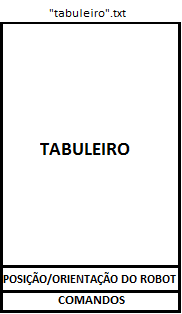
\includegraphics[scale=0.6]{./imagemdeteste.png}
    \caption{Legenda da Imagem}
    \end{center}
\end{figure}

\paragraph{}
Qualquer texto alusivo á imagem que nao a legenda da mesma deve ser colocado dentro da formatação da imagem como se pode ver no codigo tex desta imagem acima.

O texto que se segue á imagem é rescrito normalmente após o codigo de formatação da mesma (begin{figure}...end{figure}).
%++++++++++++++++++++++++++++++++++++++++++++++++++++++++++++++++++++++++++++++++++++++++++++++++++++++++++++++++++++++++++++++++++++++++++++++++++++++++++++


\newpage
\section {Criar uma bibliografia}
Quando criada uma bibliografia, esta reserva uma pagina apenas para o efeito. Assim sendo o exemplo da mesma só pode ser visto na pagina seguinte, quando, por exemplo aplicado o codigo abaixo.
\begin{verbatim}
\begin{thebibliography}{99} 
% O 99 é para indicar o maximo de numereções
\bibitem{pa}H. Partl: \emph{German \TeX}, TuGboat Volume 9,
			Issue-1 (1998)
\end{thebibliography}
\end{verbatim}

\begin{thebibliography}{99}
\bibitem {pa}H. Partl: \emph{German \TeX},TuGboat Volume 9,Issue-1 (1998)
\bibitem {pa}H. Part2: \emph{German \TeX},TuGboat Volume 9,Issue-1 (1999)

\end{thebibliography}



\end {document} % tudo o que é escrito daqui para a frente é ignorado na compilação do latex